\documentclass[usenames,dvipsnames,aspectratio=169]{beamer}
\usepackage{../common/web}

\title[Web technológiák - HTML]{Web-technológia}
\subtitle{HTML, II. rész}

\begin{document}

%1
\begin{frame}[plain]
  \titlepage
  \logoalul
\end{frame}

\section{HTML5}

%%86
\begin{frame}
  Vastag kliens alkalmazásokhoz hasonlóan adatok gyűjthetőek űrlapokkal, amiket 
  \begin{itemize}
    \item feldolgoztathatunk a szerver oldalon (most ez lesz), vagy
    \item JavaScript programmal a kliensen.
  \end{itemize}
  Űrlap vezérlők a \texttt{<form>} elembe ágyazva használhatók. Legfontosabb attribútumai:
  \begin{description}[m]
    \item[\texttt{action}] \hfill \\ A szerver oldali feldolgozó script URL-je
    \item[\texttt{target}] \hfill \\ Hova töltse a szerver válaszát 
    (\texttt{\_blank}, \texttt{\_self} (alapért.), \texttt{\_parent}, \dots)
    \item[\texttt{novalidate}] \hfill \\ Ne végezzen input 
    ellenőrzést a böngésző
    \item[\texttt{autocomplete}] \hfill \\ Korábban megadottak alapján 
    kiegészíti az adatokat (\texttt{on} (alapért.), \texttt{off})
  \end{description}
\end{frame}

%87
\begin{frame}
  \begin{description}[m]
    \item[\texttt{method}] \hfill \\ Adattovábbítási módszer:
    \begin{description}[m]
      \item[\texttt{get}] \hfill \\ Alapértelmezett. URL lekérdező 
      karakterláncában továbbítja az adatokat.
      \begin{itemize}
        \item Az URL betehető a könyvjelzők közé, és
        \item a böngészőben is könnyen szerkeszthető
      \end{itemize}
      \item[\texttt{post}] \hfill \\ HTTP tranzakcióként továbbít.
      \begin{itemize}
        \item Nincsenek méretkorlátok (URL hossza korlátozott, 
        $\approx$ 2000 karakter)
        \item Fájlok csak így továbbíthatók
        \item A böngészőben nem látszik, de ettől még \kiemel{nyílt 
        szöveg}ként továbbítják a hálózaton!
      \end{itemize}
    \end{description}
  \end{description}
\end{frame}

%88
\begin{frame}
  \begin{description}[m]
    \item[\texttt{enctype}] (type of encoding) \hfill \\ Meghatározza 
    a küldött adatok kódolását. Kötelező megadni, ha a \texttt{method} 
    attr. értéke \texttt{post}. Lehetséges értékek:
    \begin{description}[m]
      \item[\texttt{application/x-www-form-urlencoded}] \hfill \\ 
      Alapértelmezett. Minden szóközt és speciális karaktert 
      helyettesít.
      \item[\texttt{multipart/form-data}] \hfill \\ Fájlok küldésekor 
      kell használni.
      \item[\texttt{\texttt{text/plain}}] \hfill \\ Csak a szóközöket 
      helyettesíti.
    \end{description}
  \end{description}
\end{frame}

%89
\begin{frame}
  A legtöbb vezérlő az \texttt{<input>} elemmel hozható létre, pl. 
  egy számbeviteli mező néhány attribútuma, és hatása:
  \begin{description}[m]
    \footnotesize
    \item[\texttt{type}] \hfill \\ \texttt{number}, számbeviteli mező 
    létrehozása
    \item[\texttt{name}] \hfill \\ A szerver oldalon ez lesz az adat 
    \emph{kulcsa}
    \item[\texttt{min}] \hfill \\ A legkisebb bevihető érték
    \item[\texttt{max}] \hfill \\ A legnagyobb bevihető érték
    \item[\texttt{step}] \hfill \\ Ennyit változtatnak a 
    léptetőgombok/kurzurvezérlő nyilak az értéken, ennyi 
    többszöröseit lehet megadni, illetve ha 
    értéke \texttt{any}, akkor bármilyen racionális szám megadható
    \item[\texttt{required}] \hfill \\ A mező kitöltése kötelező
  \end{description}
\end{frame}

%90
\begin{frame}
  Űrlapbeküldő gomb: \texttt{<input>} elem
  \begin{itemize}
    \item \texttt{type="submit"}
    \item \texttt{value} attr. adja meg a gomb feliratát
  \end{itemize}
  \vfill
  Cimke létrehozása vezérlőhöz: \texttt{<label>} elemmel. A 
  cimkére kattintva a vezérlő is aktiválódik (pl. rádiógombnál 
  kiválasztás). Kapcsolat cimke és 
  vezérlő között:
  \begin{itemize}
    \item vezérlő a cimke belsejébe ágyazva
    \item a cimke \texttt{for} attribútumában megadható a vezérlő 
    \texttt{id}-je
  \end{itemize}
\end{frame}

%91
\begin{frame}
  Vezérlők logikai csoportosítása: \texttt{<fieldset>} elemmel\\
  Csoport feliratának megadása: \texttt{<legend>} elemben
  \vfill
  \begin{center}
    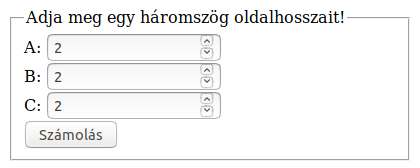
\includegraphics[width=.5\textwidth]{urlap1.png}
  \end{center}
\end{frame}

%92
\begin{frame}
  \begin{exampleblock}{\textattachfile{urlap1.html}{urlap1.html} 
  (\textattachfile{urlap1.php}{urlap1.php})}
    \footnotesize
    \lstinputlisting[style=HTML,linerange={8-20},numbers=left,firstnumber=8]{urlap1.html}
  \end{exampleblock}
\end{frame}

%%124
\begin{frame}
  A HTML5-ben beépülő modulok (pl. Flash) és akár programozás nélkül 
  lehet videót lejátszani a \texttt{<video>} elemmel (de a böngészők codec 
  támogatása hiányos). Használható formátumok:
  \begin{itemize}
    \item MP4 (video/mp4, \hiv{\href{https://caniuse.com/\#feat=mpeg4}{legjobb böngésző támogatás}})
    \item WebM (video/webm)
    \item Ogg (video/ogg)
  \end{itemize}
  Ha biztosra akarunk menni: publikálás több formátumban is.\\
  Formátumok közötti konvertálás: pl. 
  \hiv{\href{http://www.mirovideoconverter.com/}{MiroVideoConverter}}\\
  A lejátszás programozható a \hiv{\href{https://developer.mozilla.org/en-US/docs/Web/API/HTMLMediaElement}{Media API}}-val\\
\end{frame}

%125
\begin{frame}
  Ha a \texttt{<video>} elem nem támogatott egy böngészőben, a 
  címkék közötti szöveg jelenik meg. Opcionális attribútumok:
  \begin{description}[m]
    \item[\texttt{<autoplay>}] \hfill \\ A lejátszás azonnal indul; 
    \kiemel{nem ajánlott}, zavarhatja a felhasználót
    \item[\texttt{<controls>}] \hfill \\ Vezérlő gombokat jelenít meg
    \item[\texttt{<width>}, \texttt{<height>}] \hfill \\ A lejátszó 
    ablak szélessége, magassága képpontokban; \kiemel{ajánlott} megadni
    \item[\texttt{<loop>}] \hfill \\ Végtelenített lejátszás
  \end{description}
\end{frame}

%126
\begin{frame}
  \begin{description}[m]
    \item[\texttt{<muted>}] \hfill \\ Némítás
    \item[\texttt{<poster>}] \hfill \\ Egy kép, amit a betöltés 
    alatt / lejátszás megkezdéséig lát a felhasználó. Érték: URL
    \item[\texttt{<preload>}] \hfill \\ Adatfolyam betöltési módja. 
    Érték: \texttt{auto | metadata | none}.
    \item[\texttt{<src>}] \hfill \\ Videó forrása. \kiemel{Nem 
    ajánlott} a használata, mert csak egyetlen forrás nevezhető meg, 
    amit valószínűleg nem támogat minden böngésző. Érték: URL.
  \end{description}
\end{frame}

%127
\begin{frame}
  \begin{exampleblock}{\textattachfile{video1.html}{video1.html}}
    \footnotesize
    \lstinputlisting[style=HTML,linerange={8-13},numbers=left,firstnumber=8]{video1.html}
  \end{exampleblock}
    \begin{center}
    
\includegraphics[scale=.2]{video1.png}
  \end{center}
\end{frame}

%128
\begin{frame}
  Több adatforrás is megadható beágyazott \texttt{<source>} elemekkel, melyek 
  közül a böngésző az első támogatott formátumhoz tartozót 
  fogja választani. Attribútumok:
  \begin{description}[m]
    \item[\texttt{<src>}] \hfill \\ Adatforrás. Érték: URL
    \item[\texttt{<type>}] \hfill \\ A forrás MIME típusa.
  \end{description}
  A \texttt{<video>} elemmel történő kísérletezéshez egy 
  \hiv{\href{http://v4e.thewikies.com/}{érdekes eszköz}}.
\end{frame}

%129
\begin{frame}
  \begin{exampleblock}{\textattachfile{video2.html}{video2.html}}
    \scriptsize
    \lstinputlisting[style=HTML,linerange={8-22},numbers=left,firstnumber=8]{video2.html}
  \end{exampleblock}
\end{frame}

%130
\begin{frame}
  A videók feliratozhatóak is a \texttt{<track>} elemmel. Felirat 
  formátum: \hiv{\href{https://www.w3.org/TR/webvtt1/}{VTT}}. 
  \hiv{\href{https://www.nikse.dk/SubtitleEdit/Online}
  {Online szerkesztő}}, 
  \hiv{\href{https://subtitletools.com/convert-to-vtt-online}{átalakító}}. 
  Attribútumok:
  \begin{description}[m]
    \item[\texttt{<default>}] \hfill \\ Kijelölhető több feliratsáv 
    közül az alapértelmezett.
    \item[\texttt{<kind>}] \hfill \\ Feliratsáv típusa: 
    \texttt{captions | chapters | descriptions | metadata | 
    subtitles} (ez az alapértelmezés).
    \item[\texttt{<label>}] \hfill \\ Feliratsáv címkéje, pl. a 
    felirat nyelve.
    \item[\texttt{<src>}] \hfill \\ A felirat forrása, kötelező. 
    Érték: URL
    \item[\texttt{<srclang>}] \hfill \\ Felirat nyelvének ISO 639-1 
    kódja, pl. hu.
  \end{description}
\end{frame}

%131
\begin{frame}
  \begin{exampleblock}{\textattachfile{video3.html}{video3.html} 
  (\textattachfile{subtitle.vtt}{subtitle.vtt})}
    \scriptsize
    \lstinputlisting[style=HTML,linerange={8-23},numbers=left,firstnumber=8]{video3.html}
  \end{exampleblock}
\end{frame}

%132
\begin{frame}
  Feladat: készítse el a Big Buck Bunny webes lejátszóját!
  \begin{columns}[c]
    \column{0.45\textwidth}
      \begin{itemize}
        \scriptsize
        \item A videó felbontása 800x450 képpont.
        \item Poszter fotó: 
        \texttt{https://upload.wikimedia.org/wikipedia/}
        \texttt{commons/thumb/c/c5/}
        \texttt{Big\_buck\_bunny\_poster\_big.jpg/}
        \texttt{800px-Big\_buck\_bunny\_poster\_big.jpg}
        \item Két adatforrás is van, ezeket kell felajánlani: 
        \texttt{https://download.blender.org/peach/}
        \texttt{bigbuckbunny\_movies/}
        \texttt{big\_buck\_bunny\_480p\_stereo.ogg}
        és ugyanezen az útvonalon \texttt{big\_buck\_bunny\_480p\_h264.mov} 
        néven.
        \item Feliratsáv nem áll rendelkezésre.
        \item Biztosítsa a letöltés lehetőségét, ha a böngésző nem 
        támogatja a lejátszást!
      \end{itemize}      
    \column{0.45\textwidth}
      \begin{exampleblock}{\textattachfile{video4.html}{video4.html}}
        \begin{center}
          
\includegraphics[width=\textwidth]{video4.png}\\
        \end{center}
      \end{exampleblock}
  \end{columns} 
\end{frame}

%133
\begin{frame}
  Az \texttt{<audio>} elemmel lehet hangokat, zenét lejátszani. 
  Szabványos formátumok:
  \begin{itemize}
    \item MP3 (audio/mpeg, \hiv{\href{https://caniuse.com/\#feat=mp3}
    {legjobb böngésző támogatás}})
    \item Wav (audio/wav)
    \item Ogg (audio/ogg)
  \end{itemize}
  Attribútumai a méretektől eltekintve azonosak a 
  \texttt{<video>}-éival. \\
  Itt is célszerű az adatforrást beágyazott \texttt{<source>} 
  elemekkel megadni, és a lejátszást nem támogató böngészőknél 
  hibaüzenetet megjeleníteni.
\end{frame}

%134
\begin{frame}
  \begin{exampleblock}{\textattachfile{audio1.html}{audio1.html}
    (\textattachfile{dog.ogg}{dog.ogg}, 
     \textattachfile{dog.mp3}{dog.mp3})}
    \small
    \lstinputlisting[style=HTML,linerange={8-15},numbers=left,firstnumber=8]{audio1.html}
  \end{exampleblock}
  \begin{center}
    
\includegraphics[scale=.5]{audio1.png}\\
  \end{center}
\end{frame}

\subsection{Összefoglaló feladatok}


\newcounter{feladatSzamlalo}

%_
\begin{frame}
  Készítse el a \hiv{\href{https://hu.wikipedia.org/wiki/Cascading_Style_Sheets}{CSS wiki oldala}} által ihletett weblapot!
  \begin{columns}[c]
    \column{0.25\textwidth}
      \begin{exampleblock}{\textattachfile{css.html}{css.html}}
        
\includegraphics[width=\textwidth]{css1.pdf}
      \end{exampleblock}
    \column{0.75\textwidth}
      \begin{enumerate}
        \scriptsize
        \item Induljon ki a \textattachfile{css.txt}{css.txt} fájlból!
        \item Készítsen ebből magyar nyelvű HTML5 dokumentumot, UTF-8 karakterkódolással!
        \item Az oldal első szintű címsora és a böngészőfülön megjelenő szöveg egyaránt legyen ,,Cascading Style Sheets''!
        \item Ezt válassza el egy vízszintes vonallal...
        \item ...a második szintű címsorként jelölt sortól (,,A Wikipédiából, \dots'')! A ,,Tartalomjegyzék'' és az ,,Áttekintés'' szintén 2. szintű címsorként legyen jelölve!
        \item Az első bekezdés elején álló ,,CSS''-t jelölje meg rövidítésként! Ha valaki fölötte tartja az egeret, jelenjen meg a ,,Cascading Style Sheets, magyarul: lépcsőzetes stíluslapok'' szöveg egy buborékban!
        \item Jelölje meg hivatkozásként a ,,HTML'' szót, ami a megfelelő Wikipédia oldalra mutat!
        \item Járjon el ugyanígy az ,,XHTML''-lel is, de azt új fülön nyissa meg!
        \setcounter{feladatSzamlalo}{\theenumi}
      \end{enumerate}
  \end{columns}
\end{frame}

%_
\begin{frame}
  \begin{columns}[c]
    \column{0.25\textwidth}
      \begin{exampleblock}{\textattachfile{css.html}{css.html}}
        
\includegraphics[width=\textwidth]{css2.pdf}
      \end{exampleblock}
    \column{0.75\textwidth}
      \begin{enumerate}
        \footnotesize
        \setcounter{enumi}{\thefeladatSzamlalo}
        \item A dokumentum tartalma alkosson egy cikket!
        \item Minden, ami a tartalomjegyzék felett van, legyen fejlécként jelölve!
        \item Külön szakaszként jelölje a tartalomjegyzéket, és az azt követő fő fejezeteket (,,Áttekintés'', ,,A CSS használata'')!
        \item A tartalomjegyzék pontjait egymásba ágyazott, számozott listák alkossák!
        \item Ezek egyúttal legyenek hivatkozások a dokumentumon belüli fejezetekre!
        \item Az ,,Áttekintés'' fejezetben hozzon létre nem számozott felsorolást!
        \item A kötőjel előtti részt jelölje meg hangsúlyos szövegrészként!
        \item A kötőjeleket cserélje közepes hosszúságú gondolatjelekre!
        \item A felsorolás pontjaiban szereplő *-ot, HTML elemneveket, stb. jelölje meg programkódként!
        \setcounter{feladatSzamlalo}{\theenumi}
      \end{enumerate}
  \end{columns}
\end{frame}

%_
\begin{frame}
  \begin{columns}[c]
    \column{0.25\textwidth}
      \begin{exampleblock}{\textattachfile{css.html}{css.html}}
        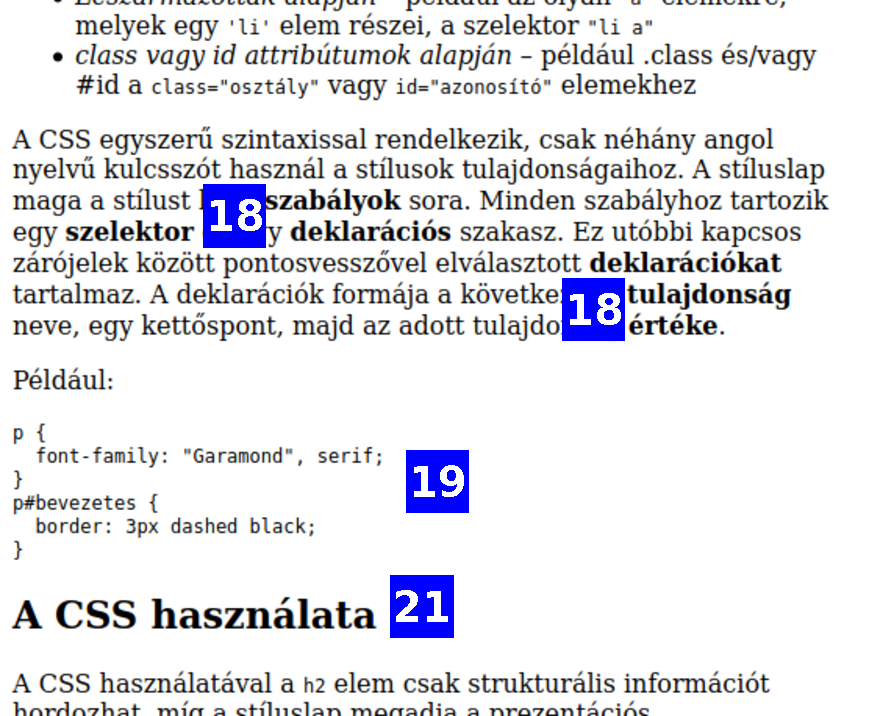
\includegraphics[width=\textwidth]{css3.pdf}
      \end{exampleblock}
    \column{0.75\textwidth}
      \begin{enumerate}
        \setcounter{enumi}{\thefeladatSzamlalo}
        \small
        \item A felsorolást követő szövegben a fontos fogalmakat (szabályok, szelektor, deklarációs, \dots) jelölje meg félkövérrel szedendő szövegként!
        \item A példaként szereplő CSS szöveget jelölje meg előformázott szövegrésznek!
        \item A CSS kód töredékeit ágyazza be olyan, előredefiniált jelentéssel nem bíró soron belüli elembe, melynek \texttt{class} attribútuma utal a kód azon részének szemantikai töltetére! A \texttt{p} elemneveknél az attribútum értéke legyen \texttt{element}, a \texttt{bevezetes}-nél \texttt{id}, a \texttt{font-family} és \texttt{border} tulajdonságnál \texttt{property}, a kettőspont utáni részeknél \texttt{keyword}, kivéve a \texttt{"Garamond"}-ot, amit jelöljön \texttt{string}-nek, a \texttt{3}-at, amit \texttt{quantity}-nak, a \texttt{px}-et pedig \texttt{unit}-nak!
        \item Jelölje meg 2. szintű címsorként ,,A CSS használata'' sort!
        \setcounter{feladatSzamlalo}{\theenumi}
      \end{enumerate}
  \end{columns}
\end{frame}

%_
\begin{frame}
  \begin{columns}[c]
    \column{0.25\textwidth}
      \begin{exampleblock}{\textattachfile{css.html}{css.html}}
        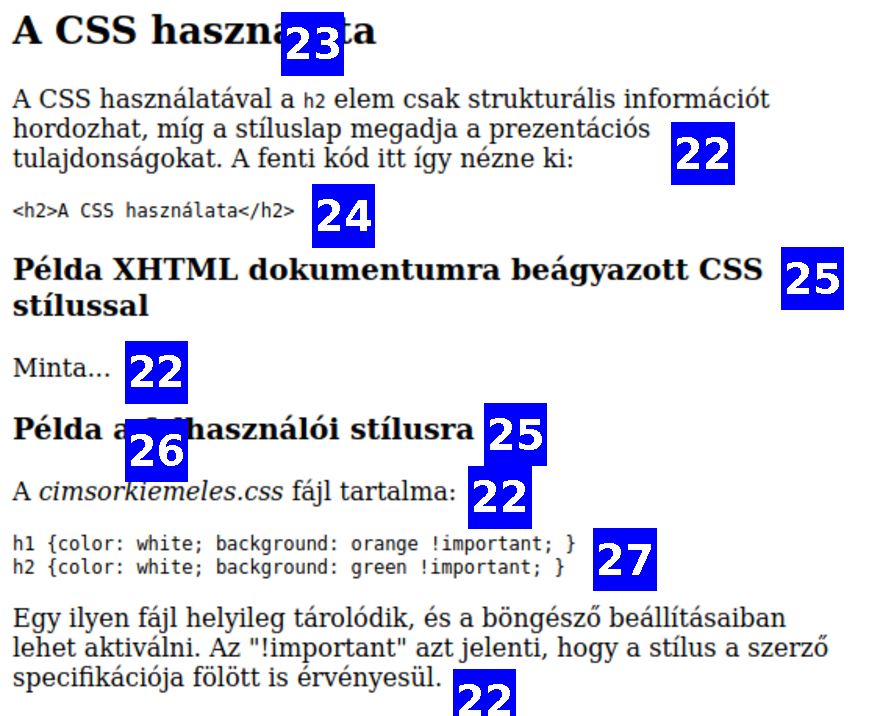
\includegraphics[width=\textwidth]{css4.pdf}
      \end{exampleblock}
    \column{0.75\textwidth}
      \begin{enumerate}
        \setcounter{enumi}{\thefeladatSzamlalo}
        \item Jelölje meg a bekezdéseket!
        \item A fejezet első bekezdésében szereplő \texttt{h2}-t jelölje meg programkódként!
        \item A következő, minta kód legyen előformázott szövegnek jelölve! Figyeljen rá, hogy minden karakter megjelenjen, és ne kezdje értelmezni azokat a böngészőprogram!
        \item Jelölje meg a ,,Példa XHTML dokumentumra\dots'' és ,,Példa a felhasználói\dots'' sorokat 3. szintű címsornak!
        \item Jelölje meg a fájlnevet dőlt betűs szövegként!
        \item A CSS szövegrészt jelölje előformázott szövegként!
        \setcounter{feladatSzamlalo}{\theenumi}
      \end{enumerate}
  \end{columns}
\end{frame}

%_
\begin{frame}
  Készítse el a \textattachfile{szamla.txt}{szamla.txt} szövegének felhasználásával az alábbi számlát!
  \begin{columns}[c]
    \column{0.5\textwidth}
      \begin{itemize}
        \small
        \item A dokumentum legyen UTF-8 kódolású, a böngészőfülön álljon \emph{Számla} felirat!
        \item Kapcsolja össze a HTML fájlt a \textattachfile{szamla.css}{szamla.css} stíluslappal!
        \item Helyezzen el a HTML fejrészében olyan leírást, amely a ,,Számla, táblázatok gyakorlásához'' szöveget tartalmazza!
        \item A számlát egy külső táblázatból, és az annak fejrészébe, törzsébe, lábrészébe beágyazott táblázatokból lehet összeállítani. Ügyeljen az általános és fejléc cellák közötti különbségekre is!
      \end{itemize}
    \column{0.5\textwidth}
      \begin{exampleblock}{\textattachfile{szamla.html}{szamla.html}}
        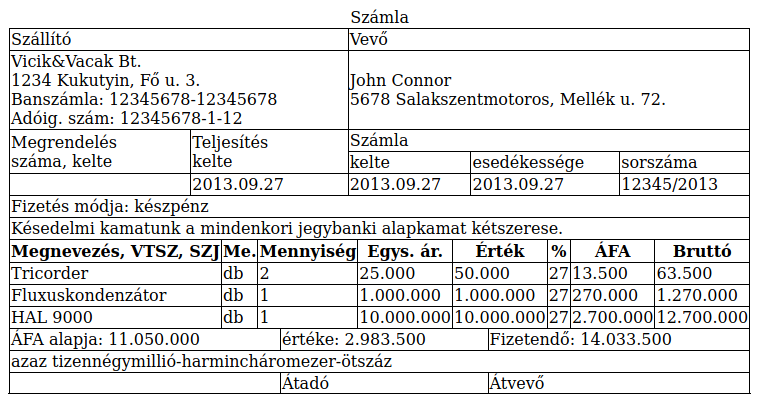
\includegraphics[width=\textwidth]{szamla.png}
      \end{exampleblock}
  \end{columns}
\end{frame}

%_
\begin{frame}
  \begin{columns}[c]
    \column{0.6\textwidth}
      Készítse el az űrlapot!
      \begin{itemize}
        \scriptsize
        \item A dokumentum legyen UTF-8 kódolású, a böngészőfülön álljon \emph{Űrlap} felirat, szövegét jelölje meg magyarként!
        \item Az űrlap tartalmát küldje \texttt{POST} módszerrel a \texttt{http://xenia.sze.hu/\textasciitilde wajzy/feldolgozo.php} címre!
        \item A beviteli mezők előtt álló magyarázó feliratok legyenek a vezérlővel összekapcsolt címkék!
        \item A ,,Név'' és ,,Életkor'' első betűit jelenítse meg félkövér betűkkel!
        \item Ezek a kiemelt betűk legyenek a vezérlő fókuszba kerülésének gyorsbillentyűi! (Többnyire \texttt{Alt+Shift+}\emph{gyorsbillentyű})
        \item Névként legfeljebb 64 karaktert lehessen bevinni, és jelenítsen meg helykitöltő szöveget arra az időre, amíg a felhasználó nem ad meg adatot!
        \item Az életkornál csak 0 és 120 közé eső számokat lehessen megadni, és kötelező kitölteni.
      \end{itemize}
    \column{0.35\textwidth}
      \begin{exampleblock}{\textattachfile{urlap.html}{urlap.html}}
        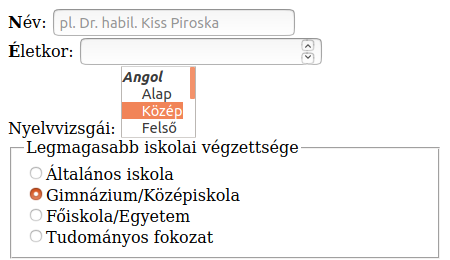
\includegraphics[width=\textwidth]{urlap-1.png}
      \end{exampleblock}
  \end{columns}
\end{frame}

%_
\begin{frame}
  \begin{columns}[c]
    \column{0.6\textwidth}
      \begin{itemize}
        \small
        \item Nyelvvizsgákból lehessen egyszerre többet is kijelölni! Angol és német nyelvből (ezek legyenek a csoportok címkéi) is lehet alap-, közép- és felsőfokú vizsgát megadni. Az angol középfok már az oldal betöltésekor legyen alapértelmezetten kiválasztva!
        \item Vegye körbe a rádiógombokat egy dobozzal, melyben a ,,Legmagasabb iskolai végzettsége'' felirat olvasható!
        \item A rádiógombok egy csoportot alkotnak, az oldal betöltésekor a ,,Gimnázium/Középiskola'' legyen kiválasztva!
      \end{itemize}
    \column{0.35\textwidth}
      \begin{exampleblock}{\textattachfile{urlap.html}{urlap.html}}
        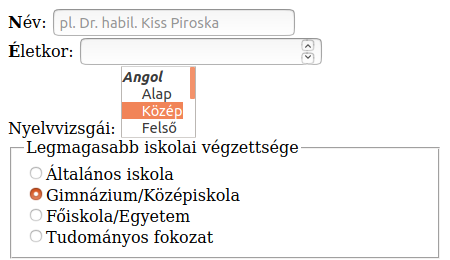
\includegraphics[width=\textwidth]{urlap-1.png}
      \end{exampleblock}
  \end{columns}
\end{frame}

%_
\begin{frame}
  \begin{columns}[c]
    \column{0.6\textwidth}
      \begin{itemize}
        \item Készítse el a hobbyk csoportját a megfelelő felirattal!
        \item Álljanak ezek jelölőnégyzetekből!
        \item A bemutatkozás szövegbeviteli mezője 40 oszlop széles, 10 sor magas legyen! Legyen benne már egy sor szöveg!
        \item Az önéletrajznál lehessen több fájlt is feltölteni egyszerre!
        \item Helyezzen el az űrlap küldésére és alaphelyzetbe állítására szolgáló gombokat!
      \end{itemize}
    \column{0.35\textwidth}
      \begin{exampleblock}{\textattachfile{urlap.html}{urlap.html}}
        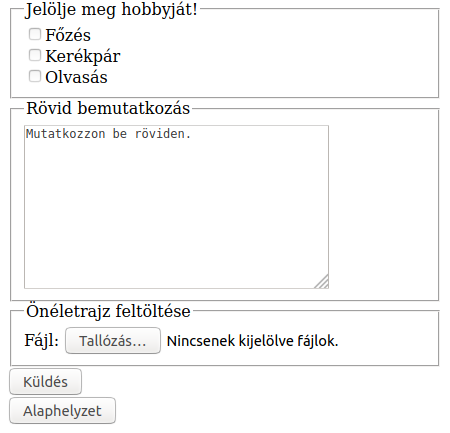
\includegraphics[width=\textwidth]{urlap-2.png}
      \end{exampleblock}
  \end{columns}
\end{frame}

%_
\begin{frame}
  Az eredmény a megadott adatoktól, a vezérlők nevétől függően az alábbihoz hasonló lehet:
  \begin{center}
    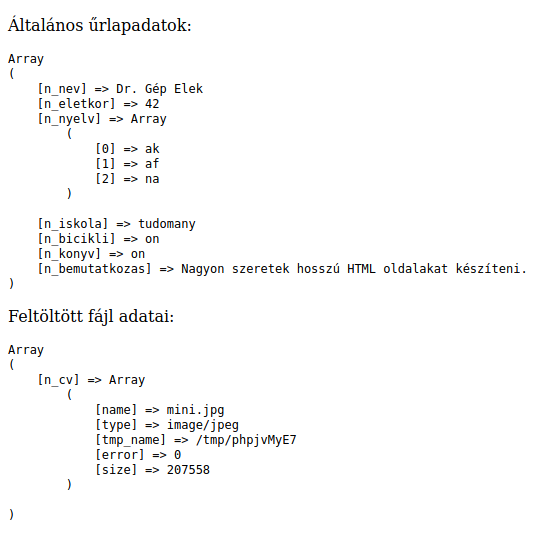
\includegraphics[width=.4\textwidth]{urlap-3.png}
  \end{center}
\end{frame}


% blokkszintű és soron belüli elemek összefoglalója
% class és id attribútumok
% Data URI

\end{document}
